
%%% \FloatBarrier
\section{Map-based Skeletons}
\label{sec:map-skeletons}
Now we have developed Parallel Arrows far enough to define some algorithmic skeletons useful to an application programmer.
\subsection{Parallel map}
\begin{figure}[h]
	\includegraphics[scale=0.7]{images/parMap}
	\caption{Schematic depiction of |parMap|.}
	\label{fig:parMapImg}
\end{figure}
The |parMap| skeleton (Fig.~\ref{fig:parMapImg},~\ref{fig:parMap}) is probably the most common skeleton for parallel programs. We can implement it with |ArrowParallel| by repeating an arrow |arr a b| and then passing it into |parEvalN| to get an arrow |arr [a] [b]|.
Just like |parEvalN|, |parMap| is 100\% strict.
\begin{figure}[h]
\begin{code}
parMap :: (ArrowParallel arr a b conf) => conf -> (arr a b) -> (arr [a] [b])
parMap conf f = parEvalN conf (repeat f)
\end{code}
\caption{Definition of parMap.}
\label{fig:parMap}
\end{figure}

\subsection{Lazy parallel map}
\begin{figure}[h]
	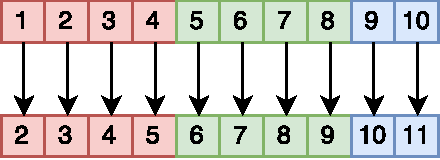
\includegraphics[scale=0.7]{images/parMapStream}
	\caption{Schematic depiction of parMapStream.}
	\label{fig:parMapStreamImg}
\end{figure}
As |parMap| (Fig.~\ref{fig:parMapImg},~\ref{fig:parMap}) is 100\% strict it has the same restrictions as |parEvalN| compared to |parEvalNLazy|. So it makes sense to also have a |parMapStream| (Fig.~\ref{fig:parMapStreamImg},~\ref{fig:parMapStream}) which behaves like |parMap|, but uses |parEvalNLazy| instead of |parEvalN|.
\begin{figure}[h]
\begin{code}
parMapStream :: (ArrowParallel arr a b conf, ArrowChoice arr, ArrowApply arr) =>
	conf -> ChunkSize -> arr a b -> arr [a] [b]
parMapStream conf chunkSize f = parEvalNLazy conf chunkSize (repeat f)
\end{code}
\caption{Definition of |parMapStream|.}
\label{fig:parMapStream}
\end{figure}

\subsection{Statically load-balancing parallel map}
\begin{figure}[h]
	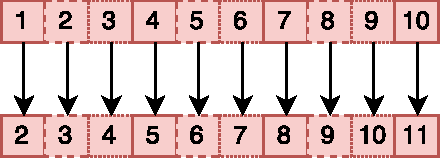
\includegraphics[scale=0.7]{images/farm}
	\caption{Schematic depiction of a |farm|, a statically
          load-balanced |parMap|.}
	\label{fig:farmImg}
\end{figure}
A |parMap| (Fig.~\ref{fig:parMapImg},~\ref{fig:parMap}) spawns every single computation in a new thread (at least for the instances of |ArrowParallel| we gave in this paper). This can be quite wasteful and a |farm| (Fig.~\ref{fig:farmImg},~\ref{fig:farm}) that equally distributes the workload over |numCores| workers (if numCores is greater than the actual processor count, the fastest processor(s) to finish will get more tasks) seems useful.
The definitions of helper functions |unshuffle|, |takeEach|, |shuffle| (shown in Appendix) originate from an Eden skeleton\footnote{Available on Hackage under \url{https://hackage.haskell.org/package/edenskel-2.1.0.0/docs/src/Control-Parallel-Eden-Map.html}.}.
\begin{figure}[h]
\begin{code}
farm :: (ArrowParallel arr a b conf,
	ArrowParallel arr [a] [b] conf, ArrowChoice arr) =>
	conf -> NumCores -> arr a b -> arr [a] [b]
farm conf numCores f =
	unshuffle numCores >>>
	parEvalN conf (repeat (mapArr f)) >>>
	shuffle

unshuffle :: (Arrow arr) => Int -> arr [a] [[a]]
unshuffle n = arr (\xs -> [takeEach n (drop i xs) @|@ i <- [0..n-1]])

takeEach :: Int -> [a] -> [a]
takeEach n [] = []
takeEach n (x:xs) = x : takeEach n (drop (n-1) xs)

shuffle :: (Arrow arr) => arr [[a]] [a]
shuffle = arr (concat . transpose)
\end{code}
\caption{The definition of |farm|.}
\label{fig:farm}
\end{figure}

\subsection{The |farmChunk| Skeleton}
\begin{figure}[h]
	\includegraphics[scale=0.7]{images/farmChunk}
\caption{Schematic depiction of farmChunk.}
\label{fig:farmChunkImg}
\end{figure}
Since a |farm| (Fig.~\ref{fig:farmImg},~\ref{fig:farm}) is basically just |parMap| with a different work distribution, it is, again, 100\% strict. So we can define |farmChunk| (Fig.~\ref{fig:farmChunkImg},~\ref{fig:farmChunk}) which uses |parEvalNLazy| instead of |parEvalN|. It is basically the same definition as for |farm|, with |parEvalN| replaced with |parEvalNLazy|, as Appendix shows.

\subsection{Map and reduce}

A~simple |map|--|reduce| can be written like in Figure~\ref{fig:parMapReduceDirect}. Notice that the performance of the |>>>| combinator is essential for the performance of the skeleton. A~definitive version would use Futures.

 \olcomment{it appears STRANGE. are the data really left alone and noded after map and taken from there by reduce? It makes sense only is no communication through master takes place. ELSE: CUT!}


 \mbcomment{this requires some work. Either change this to use futures or cut, yes.}
% -- this does not completely adhere to Google's definition of Map Reduce as it
% -- the mapping function does not allow for "reordering" of the output
% -- The original Google version can be found at https://de.wikipedia.org/wiki/MapReduce

\olcomment{now rewritten as motivation for futures. maybe still cut?}

\begin{figure}[h]
\begin{code}
parMapReduceDirect :: (ArrowParallel arr [a] b conf, ArrowApply arr, ArrowChoice arr) =>
	conf -> ChunkSize -> arr a b -> arr (b, b) b -> b -> arr [a] b
parMapReduceDirect conf chunkSize mapfn foldfn neutral =
	arr (chunksOf chunkSize) >>>
	parMap conf (mapArr mapfn >>> foldlArr foldfn neutral) >>>
	foldlArr foldfn neutral
\end{code}
\caption{Definition of parMapReduceDirect.}
\label{fig:parMapReduceDirect}
\end{figure}


%%% Local Variables:
%%% mode: latex
%%% TeX-master: "main"
%%% End:
